\documentclass[10pt]{beamer}
\title{DOMinating the Web}
\author{Eric Wood}
\date{October 9, 2012}

\usepackage{graphicx}
\usepackage{listings}
\usepackage{minted}
\usepackage{fancyvrb}
\usepackage{color}
\usepackage{hyperref}

\usemintedstyle{pastie}

\graphicspath{{./images}}

\usetheme{Copenhagen}
\usecolortheme{beaver}
\setbeamertemplate{items}[ball]

% TODO: come back and play with these later!
%\definecolor{darkgrey}{RGB}{23,23,23}
%\definecolor{lightgrey}{RGB}{193,193,193}
%\setbeamercolor{frametitle}{fg=blue}
%\setbeamercolor*{palette primary}{bg=gray}

\begin{document}

\maketitle

%\frame
%{
%  \frametitle{Table of Contents}
%  \tableofcontents
%}

\section{Introduction}
\subsection{History}
\frame
{
  \frametitle{A brief history of web development}
  \begin{itemize}
    \item (1989) Tim Berners-Lee comes up with the idea of HTML for use at CERN and basically gives birth to the modern interwebs
    \item (1993) First HTML spec defined by the Internet Engineering TaskForce (IETF)
    \item (1994) The World Wide Web Consortium (W3C) is formed by Berners-Lee.
    \item (1994) Tim Berners-Lee names himself "Supreme Internet Overlord"
    \item (present) Everything is a mess, but things are looking up!
  \end{itemize}

  \emph{ALL HAIL THE SUPREME INTERNET OVERLORD!}
}

\subsection{What are web pages made of?}
\frame
{
  \frametitle{Web pages: what are they made of?}

  \begin{description}
    \item[HTML - HyperText Markup Language] \hfill \\
      The page's content and basic structure
    \item[CSS - Cascading Style Sheets] \hfill \\
      Controls the page's style and presentation
    \item[JavaScript] \hfill \\
      Scripting language for manipulating the above, amongst other things...
  \end{description}
}

\section{HyperText Markup Language (HTML)}
\subsection{The Basics}
\frame
{
  \frametitle{The Basics}

  \begin{itemize}
    \item Collection of "tags"
      \begin{itemize}
        \item \lstinline|<b>this text is now bold LOL</b>|
      \end{itemize}
    \item Tags can be nested
      \begin{itemize}
        \item \lstinline|<i><b>this text is now bold *and* italic...whoa...</b></i>|
      \end{itemize}
    \item Tags can have attributes
      \begin{itemize}
        \item \lstinline|<a href="http://ericwood.org">This is an "anchor" tag</a>|
      \end{itemize}
  \end{itemize}
}

\frame
{
  \frametitle{The Basics}

  \begin{quotation}
    At some point in the evening I mentioned that it was sad that Lynx was not going to be able to display many of the HTML extensions that we were proposing, I also pointed out that the only text style that Lynx could exploit given its environment was blinking text. We had a pretty good laugh at the thought of blinking text, and talked about blinking this and that and how absurd the whole thing would be. [...] Saturday morning rolled around and I headed into the office only to find what else but, blinking text. It was on the screen blinking in all its glory, and in the browser. How could this be, you might ask? It turns out that one of the engineers liked my idea so much that he left the bar sometime past midnight, returned to the office and implemented the blink tag overnight. He was still there in the morning and quite proud of it.
  \end{quotation}
  - Lou Montulli (creator of Lynx)
}

\subsection{Important Attributes and Tags}
\frame
{
  \frametitle{Important Attributes and Tags}

  \begin{itemize}
    \item \lstinline|<div>| and \lstinline|<span>| tags are for dividing up portions of the document (more on this later)
    \item The ID attribute gives a tag a unique identifier to make it easy to find: \lstinline|<div id="foobar">|
    \item The class attribute identifies multiple tags: \lstinline|<div class="foobar">|
  \end{itemize}
}

\subsection{The Document Object Model (DOM)}
\frame
{
  \frametitle{The Document Object Model (DOM)}

  \begin{itemize}
    \item All of these tags form a tree structure called the DOM tree
    \item The root node is considered the "document"
    \item JavaScript traverses and modifies nodes in the DOM tree
    \item Note that the DOM is an abstraction that applies to other markup languages as well (XML, SGML, etc.)
  \end{itemize}
}

\subsection{Example HTML Document}
\begin{frame}[fragile]
  \frametitle{Example HTML Document}

  \inputminted{html}{./code/html_example.html}
\end{frame}

\section{Cascading Style Sheets (CSS)}
\subsection{Selectors}
\frame
{
  \frametitle{Selectors}

  Selectors are a syntax for selecting nodes in the DOM tree
  Here's some awesome examples:
  \begin{itemize}
    \item \lstinline|b| (all \lstinline|<b>| tags)
    \item \lstinline|.foo| (all nodes with \lstinline|class="foo"|)
    \item \lstinline|\#foo| (all nodes with \lstinline|id="foo"|)
    \item \lstinline|b.foo| (all \lstinline|<b>| tags with \lstinline|class="foo"|)
    \item \lstinline|\#foo b| (every \lstinline|<b>| tag inside a node with \lstinline|id="foo"|)
    \item Enumerating them sucks. Live code??
  \end{itemize}
}

\subsection{Attributes}
\frame
{
  \frametitle{Attributes}

  \begin{itemize}
    \item Elements have style attributes which are set via CSS
    \item Too many to discuss here, but I'll touch on them as I progress
    \item Here's an example thingy:
  \end{itemize}

  \inputminted{css}{./code/css_attrs.css}
}

\subsection{Positioning and the Box Model}
\frame
{
  \frametitle{Positioning and the Box Model}

  BOW BEFORE THE GLORIOUS BOX MODEL.

  \begin{center}
    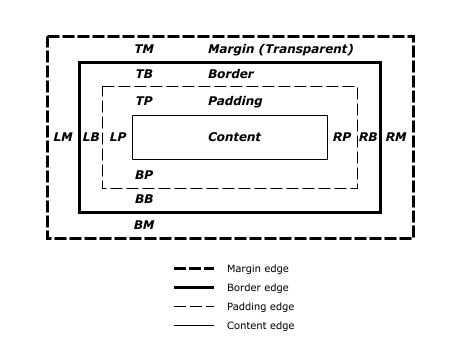
\includegraphics[scale=0.65]{./images/box_model.png}
  \end{center}
}

\frame
{
  \frametitle{Positioning and the Box Model}

  \begin{itemize}
    \item Block-level elements
      \begin{itemize}
        \item \lstinline|<div>|, \lstinline|<p>|, etc.
        \item Elements above and below are on new lines
      \end{itemize}
    \item Inline elements
      \begin{itemize}
        \item \lstinline|<span>|, \lstinline|<b>|, \lstinline|<i>|, etc.
        \item Appear inline with their surrounding elements; no automatic spacing or whatever
      \end{itemize}
  \end{itemize}
}


\subsection{The Cascade}
\frame
{
  \frametitle{The Cascade}

  \begin{itemize}
    \item The "cascade" part of the acronym refers to the way inheritance works
    \item CSS rules can be defined in several parts of the document and almost always overlap
    \item So...how exactly do elements inherit their styles?
    \item Lets discuss the pecking order!
  \end{itemize}
}

\frame
{
  \frametitle{The Cascade}

  \begin{enumerate}
    \item Gather all selectors that apply to an element
    \item Order them based on the following criteria:
      \begin{enumerate}
        \item Source (ascending order)
          \begin{enumerate}
            \item Browser defaults
            \item Author's stylesheets
          \end{enumerate}
        \item Specification method
          \begin{enumerate}
            \item Linked stylesheet
            \item Embedded stylesheet (\lstinline|<style| tag)
            \item Inline styles (style attribute on the tag itself)
          \end{enumerate}
        \item Element selector specificity
          \begin{enumerate}
            \item Contextual selector depth
            \item Class
            \item ID
          \end{enumerate}
        \item The \lstinline|!important| flag
      \end{enumerate}
    \item Sort by order specified
  \end{enumerate}
}

\subsection{Putting it all together}
\frame
{
  \frametitle{Putting it all together}

  Live demo time. Lets build a badass webpage \emph{from scratch} :D
}

\section{JavaScript}
\subsection{Fundamentals}
\frame
{
  \frametitle{Fundamentals}

  \begin{itemize}
    \item JavaScript falls into the following programming language paradigms:
      \begin{itemize}
        \item Object-oriented (classless aka. prototyped) - not like C++, mmk?
        \item Functional (I hope you like anonymous functions!!!!)
        \item Imperative (the paradigm you're most familiar with)
      \end{itemize}
    \item Dynamic typing
    \item Objects are everything
  \end{itemize}
}

\frame
{
  \frametitle{Objects}

  \begin{itemize}
    \item Pretty much everything is an object
    \item Basically a key-value store (a hash map, if you prefer that term)
    \item Prototypes
      \begin{itemize}
        \item More advanced and beyond the scope of this talk
        \item You won't use them very often unless you're really awesome
        \item These are how inheritance and OOP happens in JS
      \end{itemize}
  \end{itemize}
}

\frame
{
  \frametitle{Functions}
  
  \begin{itemize}
    \item JS functions are \emph{first-class} -- they're treated like data (this is the definition of functional programming, omg)
    \item You can give them names, or define them inline as anonymous functions
  \end{itemize}
}

\subsection{The DOM API}
\frame
{
  \frametitle{Messin' with the DOM}

  \begin{itemize}
    \item Very simple, but kind of powerful I guess
    \item The "document" JS object provides a means for accessing attributes and modifying the DOM tree
    \item \lstinline|document.getElementById()|
    \item \lstinline|document.getElementsByClassName()|
    \item The \lstinline|Element| object provides access to tag attributes and functions for DOM traversal from that node in the tree
    \item Complete reference: \url{https://developer.mozilla.org/en-US/docs/DOM/element}
  \end{itemize}
}

\frame
{
  \frametitle{Caveats}

  \begin{itemize}
    \item Lots of manual traversal (lame)
    \item If I need to modify attributes on a set of nodes I have to iterate over them
    \item Inconsistent between browsers (this applies to all aspects of web dev, though)
  \end{itemize}
}

\frame
{
  \frametitle{Is there a solution?!}

  A very emphatic \emph{yes}. jQuery to the rescue!

  \begin{itemize}
    \item jQuery is a JS library that provides a developer-friendly (and cross-browser!) means for interacting with the DOM
    \item There are many other libraries (Prototype, Mootools, etc.), but I \lstinline|<3| jQuery the most (as do a majority of web devs), so I'll focus on it for the rest of this talk
  \end{itemize}

  \begin{center}
    
\includegraphics[scale=0.2]{./images/jquery_logo.png}
  \end{center}
}

\subsection{jQuery}
\frame
{
  \frametitle{The jQuery Object}

  \begin{itemize}
    \item The \lstinline|$| function is used by jQuery for everything
    \item We can use the \lstinline|$()| function along with CSS selectors to grab elements
      \begin{itemize}
        \item \lstinline|$('\#foo')|, etc.
        \item jQuery returns the result as an array object with additional functionality; this allows us to modify multiple nodes in a single function call! In the background it takes care of the iteration and DOM API calls for us
      \end{itemize}
    \item The \lstinline|$()| function can also generate new nodes
      \begin{itemize}
        \item \lstinline|$('<div/>');| returns a brand new \lstinline|<div>| tag
      \end{itemize}
    \item Appending and modifying the DOM tree is easy with wrapper methods like \lstinline|appendTo()|
  \end{itemize}
}

\subsection{Event Handling}
\frame
{
  \frametitle{Event Handling}

  \begin{itemize}
    \item We can use jQuery event handlers to wrap the normal and less awesome DOM API
    \item JS is well-suited to event-driven programming in its use of functional programming
  \end{itemize}

  Lets try out a few event handlers!
}

\subsection{AJAX}
\frame
{
  \frametitle{AJAX - the buzzword we hate to love}

  \begin{itemize}
    \item AJAX is a stupid acronym for Asynchronous JavaScript And XML
    \item It has nothing to do with XML, but it \emph{is} asynchronous
    \item The \lstinline|XMLHttpRequest| function allows us to retrieve content from a remote server
      \begin{itemize}
        \item The content must come from the same server the page was loaded from for security reasons (same-origin policy)
      \end{itemize}
    \item People usually prefer JSON (JavaScript Object Notation) over XML since it's more complex and is actually valid JS code
  \end{itemize}
}

\frame
{
  \frametitle{AJAX with XMLHttpRequest Example}

  \inputminted{javascript}{./code/xmlhttprequest.js}
}

\frame
{
  \frametitle{AJAX in jQuery}

  \begin{itemize}
    \item \lstinline|$.ajax()| is a handy function that wraps XMLHttpRequest in a friendly manner
    \item Reduces the complexity of handling errors with XMLHttpRequest
    \item Automatically parse JSON securely
  \end{itemize}
}

\section{Putting it all together}
\frame
{
  \frametitle{Putting it all together}

  Example time!
}

\section{Resources}
\frame
{
  \frametitle{Useful resources}
  \begin{itemize}
    \item \underline{\href{''https://developer.mozilla.org/en-US/''}{Mozilla Developer Network}} - the everything reference
    \item \underline{\href{''http://www.quirksmode.org/''}{quirksmode.org}} - the most comprehensive browser compatibility tables in the universe
    \item \underline{\href{''http://www.w3.org/standards/webdesign/''}{W3C Standards}} - the \emph{official} specifications for HTML, CSS, and JavaScript
  \end{itemize}
}

\end{document}
